\documentclass[aspectratio=169,graphics,handout]{beamer} 

\usepackage[]{minted}
\usepackage{Preamble}
\usepackage{forloop}

\graphicspath{{./img/}}

\newcommand{\proarg}{\item[\textbf{+}]}
\newcommand{\contraarg}{\item[\textbf{-}]}

\title[12.04.2024 - Sustainable Scientific Software Development]{Sustainable Scientific Software Development}
\author[Schlemmer, Wellecke, Kottlarz]{Alexander Schlemmer, Gerrit Wellecke, Inga Kottlarz}
\institute{} 
\date{12.04.2024}

\begin{document}
% has to be loaded outside of a frame to work!
\maketitle

\begin{frame}{Introduction}
    \begin{itemize}
        \item Alexander Schlemmer
        \item Gerrit Wellecke
        \item Inga Kottlarz
    \end{itemize}
\end{frame}

\begin{frame}{About the topic: What is "Sustainable Software"?}
    The term "sustainable" can have two meanings in this context:
    \begin{itemize}
        \item Green IT (e.g. energy consumption)\footnote{\url{https://en.wikipedia.org/wiki/Green_computing}}
        \item Software that is maintainable, extendable, documented and re-usable\footnote{See e.g.: Blech C, Dreyer N, Friebel M, et al (2022) SURESOFT: Towards Sustainable Research Software 10.24355/dbbs.084-202210121528-0} %FIX: \cite{dbbs_mods_00071451}}
    \end{itemize}

    No stable definition so far.

    % We will mostly talk about the latter. But the contents of this course also have a high impact on
    % green IT: Energy saved when software is easily re-usable. Bugs can be found faster. Profiling saves energy.
\end{frame}


\begin{frame}{About the topic: What is "Sustainable Software"?}

    \begin{block}{@chatgpt Can you define Software development?}

        Software development is the process of conceiving, specifying, designing, programming, documenting, testing, and bug fixing involved in creating and maintaining applications, frameworks, or other software components.
    \end{block}

\end{frame}

\begin{frame}{Software development in research}
    What is so special about research software?

    \begin{itemize}
        \item ... often developed by scientists, but not by professional software engineers
        \item ... has a special (and specialized) target group
        \item Very small software development "teams".
        \item Limited contracts and third-party funding impede long-term maintenance.
    \item ... with rather "short-term goals in mind" %FIX: \cite{dbbs_mods_00071451}
\end{itemize}
\end{frame}

\begin{frame}{(Prototype-)Scripting vs. Software Development}
    Pros and cons of scripts:
    \begin{itemize}
        \proarg Quick'n'dirty / Prototypes
        \proarg Exploratory projects
        \proarg Interactivity, e.g. Jupyter Notebooks
        \pause
        \contraarg Usability
        \contraarg Lack of documentation, testing
        \contraarg Very specific (often hard-coded) use-case
        \contraarg Difficult to maintain
\end{itemize}

\end{frame}

\begin{frame}{Typical Scenarios}
    \begin{itemize}
        \item Software developed during PhD. Outstanding method (scientifically), but developed with poor software development skills.
        \item[$\rightarrow$] Software is unmaintainable and will not be used beyond the scope of the PhD thesis.

            \pause

        \item Software developed during grant for 3 years. Software is not published after the end of the grant. Furthermore, no documentation.
        \item[$\rightarrow$] Software is no longer usable beyond the scope of the grant.
    \end{itemize}

\end{frame}

\begin{frame}{Contents of this course}
    \begin{enumerate}
        \item git / gitlab / version control (2 sessions)
            \pause
        \item packaging / project management (2 sessions)
            \pause
        \item design patterns / programming paradigms
            \pause
        \item automated testing (2 sessions)
            \pause
        \item documentation
            \pause
        \item debugging
            \pause
        \item profiling
            \pause
        \item software development workflows in science
            \pause
        \item publishing software / open source licenses
            \pause
        \item AI tools
    \end{enumerate}
\end{frame}

\begin{frame}{Programming languages}
    \begin{itemize}
        \item Our policy: Use your favorite programming language.
        \item Lingua franca: Python
        \item Most popular languages in research: Python, R, Matlab, Julia
        \item Performance / low level hardware access: C/C++, Rust, (Assembler)
        \item Web languages: JavaScript, (HTML, CSS), PHP
        \item Programming language popularity indices: TIOBE\footnote{https://www.tiobe.com/tiobe-index/}, pypl\footnote{https://pypl.github.io/PYPL.html}
    \end{itemize}
\end{frame}

\begin{frame}{Data formats}

    %TODO: Do we need this slide? I want to mention that markdown and yaml is needed.
    \begin{itemize}
        \item XML
        \item YAML
        \item JSON
        \item Markdown
    \end{itemize}
\end{frame}

\begin{frame}{XML}
    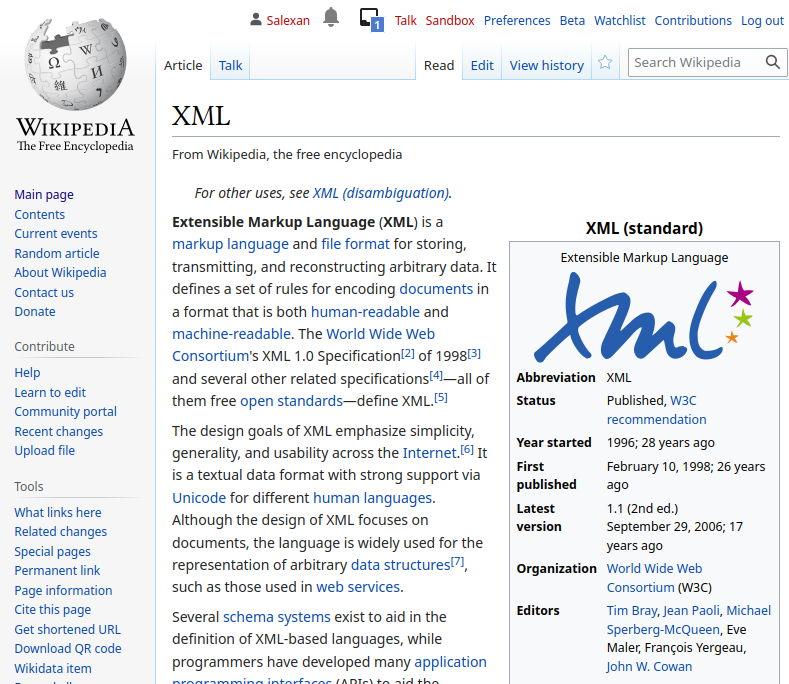
\includegraphics[width=\textwidth]{xml.png}
\end{frame}


\begin{frame}[fragile]{Example: XML}
    (ChatGPT): Certainly! Here's a simple XML example that could be used to represent information about a book in a library system:

    \begin{minted}{xml}
<?xml version="1.0" encoding="UTF-8"?>
<book>
  <title>The Great Gatsby</title>
  <author>F. Scott Fitzgerald</author>
  <year>1925</year>
  <genre>Fiction</genre>
  <publisher>Charles Scribner's Sons</publisher>
</book>
    \end{minted}

    This XML document includes basic information about the book, such as its title, author, publication year, genre, and publisher.
\end{frame}

\begin{frame}{YAML}
    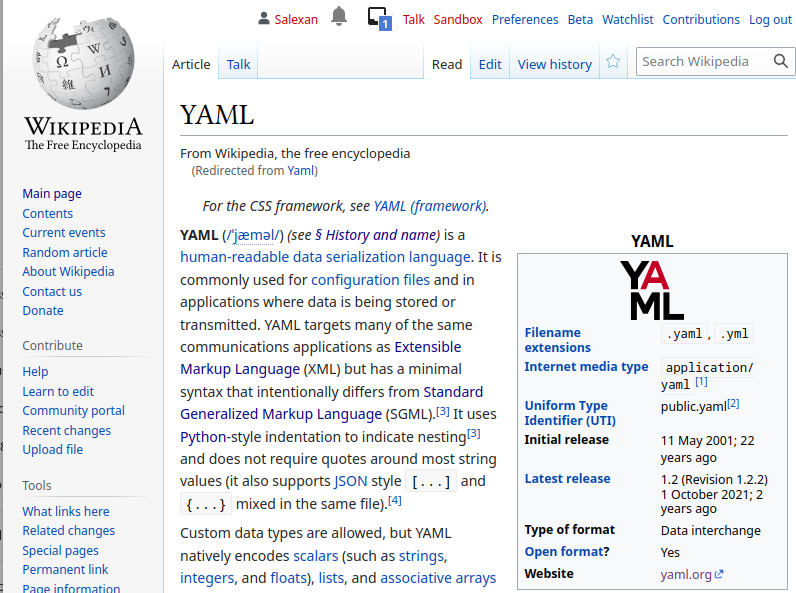
\includegraphics[width=\textwidth]{yaml.png}
\end{frame}

\begin{frame}[fragile]{Example: YAML}
\begin{minted}{yaml}
book:
  title: The Great Gatsby
  author: F. Scott Fitzgerald
  year: 1925
  genre: Fiction
  publisher: Charles Scribner's Sons
\end{minted}
\end{frame}

\begin{frame}{JSON}
    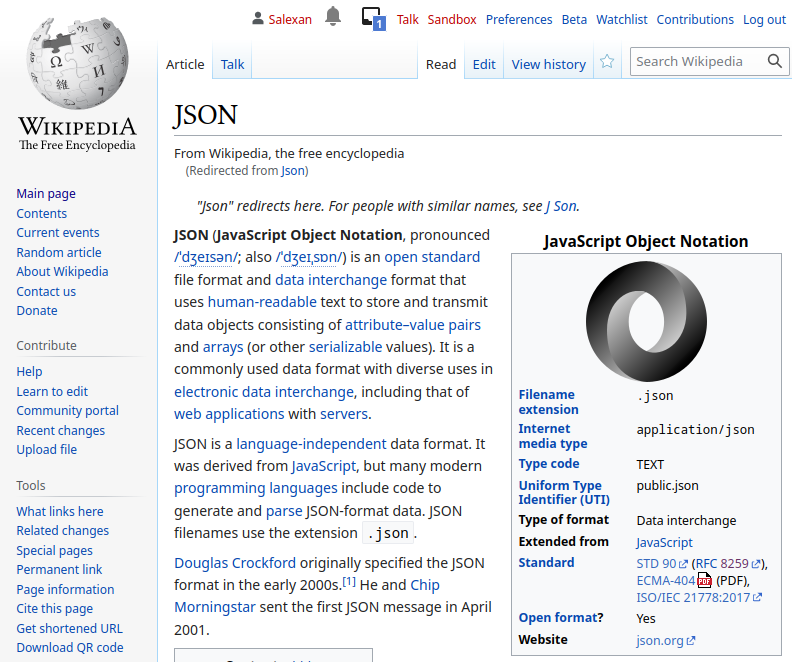
\includegraphics[width=\textwidth]{json.png}
\end{frame}

\begin{frame}[fragile]{Example: JSON}
    \begin{minted}{json}
{
  "book": {
    "title": "The Great Gatsby",
    "author": "F. Scott Fitzgerald",
    "year": 1925,
    "genre": "Fiction",
    "publisher": "Charles Scribner's Sons"
  }
}
    \end{minted}
\end{frame}

\begin{frame}{Markdown}
    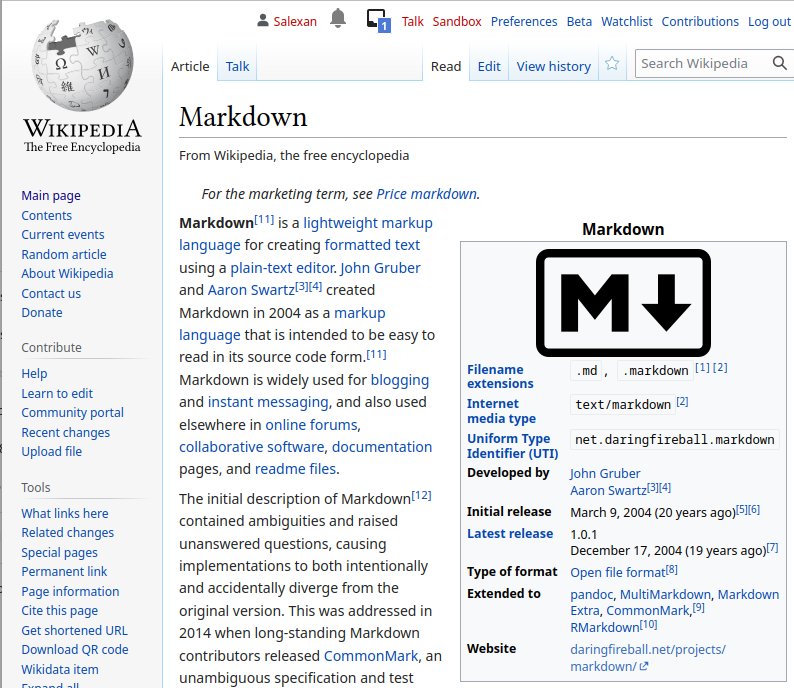
\includegraphics[width=\textwidth]{markdown.png}
\end{frame}

\begin{frame}[fragile]{Example: Markdown 1}
\begin{minted}{markdown}
# Book Information

- **Title:** The Great Gatsby
- **Author:** F. Scott Fitzgerald
- **Year:** 1925
- **Genre:** Fiction
- **Publisher:** Charles Scribner's Sons
\end{minted}
\end{frame}

\begin{frame}[fragile]{Example: Markdown 2}
\begin{minted}{markdown}
---
title: "The Great Gatsby"
author: "F. Scott Fitzgerald"
year: 1925
genre: "Fiction"
publisher: "Charles Scribner's Sons"
---

# The Great Gatsby

Text follows here.

\end{minted}
\end{frame}

\begin{frame}{Python}
    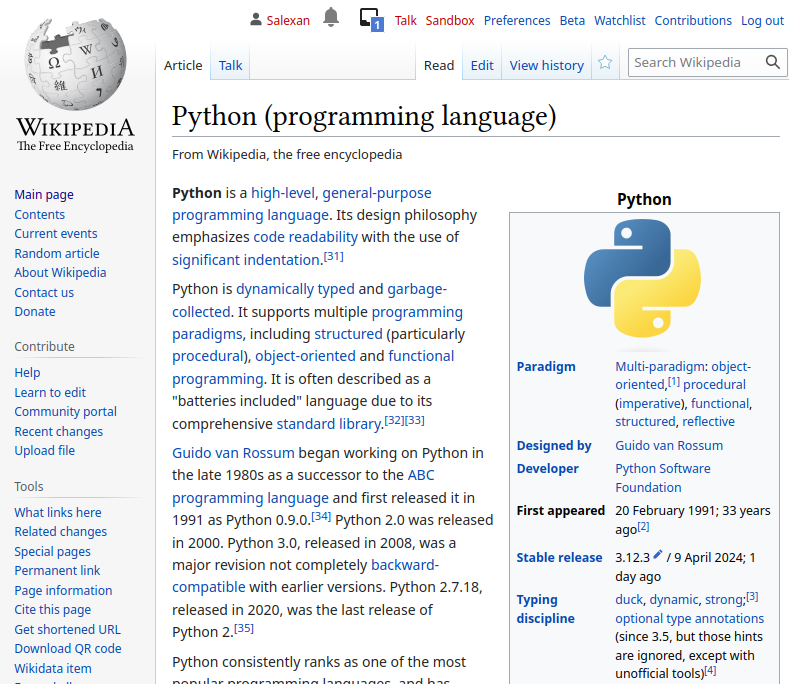
\includegraphics[width=\textwidth]{python.png}
\end{frame}

\begin{frame}{Jupyter notebooks}

    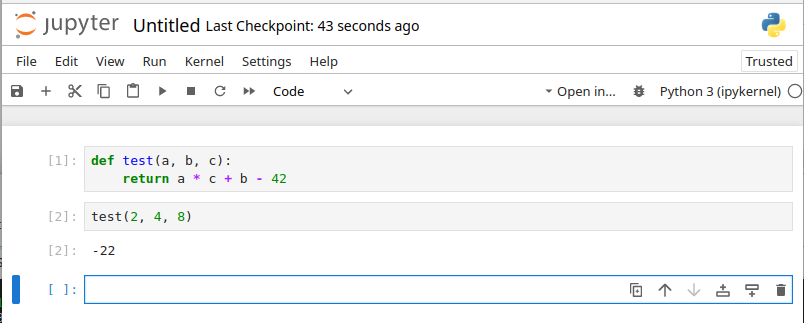
\includegraphics[width=\textwidth]{screenshot_jupyter.png}
    % What is it?
    % What are they suited for?
    % Why are they not suited for software development?
\end{frame}

\begin{frame}{Jupyter notebooks}

    \begin{itemize}
        \item Interactive notebooks for multiple programming languages:\\
            JUlia PYThon R (but also others)
        \item Runs in the browser and communicates with interactive kernels
        \item Useful for: (Prototype-)Scripting, Try-and-error-workflows, documentation of scientific work
        \item Absolutely not recommended for sustainable software development:\\
            Main problem: nonlinear evaluation of cells.
    \end{itemize}
\end{frame}

\begin{frame}{IDEs and editors}
    \begin{itemize}
        \item Policy: Use your favorite editor / IDE!
        \item Some recommendations:
            \begin{itemize}
                \item Emacs / Vim
                \item VSCode / VSCodium\footnote{https://vscodium.com/}
            \end{itemize}
    \end{itemize}
\end{frame}

\begin{frame}{Model system: Game of Life}
    % Show wikipedia page with many examples.
    \begin{itemize}
        \item "Conway's Game of Life"
        \item {\small \url{https://en.wikipedia.org/wiki/Conway\%27s_Game_of_Life}}
        \item Cell-automaton with few rules
        \item Generates complex self-sustaining patterns
        \item Try it out: \url{https://playgameoflife.com/}
        \item Interesting documentary (about Turing completeness of Game of Life):
            {\small \url{https://www.youtube.com/watch?v=Kk2MH9O4pXY&list=TLPQMDUwNDIwMjTwyHzmJBFbDQ&index=1} Alan Zucconi - "Let's build a Computer in Conway's Game of Life"}
    \end{itemize}

    % In die Tiefe gehen...
    % active research
    % long stable periodic orbits
    % Turing complete
\end{frame}

\begin{frame}{Technical Requirements of this Course}
    \begin{itemize}
        \item Computer
        \item git + ssh
        \item Any IDE or text editor
        \item Running Python or your favorite programming language
        \item University or GWDG-account for gitlab
        \item Web browser :-)
    \end{itemize}

    % Windows: Tortoise GIT? oder WSL
    % https://tortoisegit.org/
\end{frame}


\begin{frame}{Formalities of this course}

    \begin{block}{Oral exam / FlexNow}
        \begin{itemize}
            \item For Bachelor/Master-students
            \item Please register in FlexNow: 7 days before 2024-09-30!
            \item 20min.
        \end{itemize}
    \end{block}

    \pause

    \begin{block}{StudIP}
        Please enroll in the StudIP course!
    \end{block}

    \pause

    \begin{block}{Remote}
        Remote participation is possible in exceptional cases (e.g. child-care). Please write us an email.
    \end{block}

\end{frame}

\begin{frame}{gitlab-Workflow}
    \begin{itemize}
        \item Create your fork of our repository on gwdg-gitlab (gitlab.gwdg.de).
        \item Develop your code in the tutorial session.
        \item Exercise code-review in small groups and create a merge request in \textbf{our} repository until Wednesday of the next week.
        \item We choose one version to keep in the main repository.
        \item More details next week.
    \end{itemize}

    \pause
    \begin{block}{Goal}
        Create a software package for Game of Life.
    \end{block}

\end{frame}

\begin{frame}{Discussion}
    \begin{itemize}
        \item Are there topics of interest, we have forgotten?
        \item Previous experience with these topics?
    \end{itemize}
\end{frame}

\begin{frame}[t,allowframebreaks]{Literature}
    \printbibliography{}
\end{frame}

% Teaser für Themen, z.B. "debugging", "design patterns"
% Gibt es Themen, die euch besonders interessieren? Oder die wir vergessen haben?
% Habt ihr schon mal mit diesen Dingen zu tun gehabt?



\end{document}
